\documentclass[12pt]{article}
\usepackage[utf8]{inputenc}
\usepackage{amsmath}
\usepackage{graphicx}
\usepackage{float}
\usepackage{dsfont}
\usepackage{tikz,lipsum,lmodern}
\usepackage[most]{tcolorbox}
\usepackage{textcomp}
\usepackage{multirow}
\usepackage{amsfonts}
\usepackage[nottoc,numbib]{tocbibind}
\usepackage{hyperref}
\usepackage{cleveref}
\usepackage{fancyhdr}
\setlength{\headheight}{14.5pt}
\renewcommand{\sectionmark}[1]{\markright{#1}{}}
\usepackage[T1]{fontenc}
\usepackage[colorinlistoftodos]{todonotes}
\usepackage[margin=2cm,a4paper]{geometry}
\newgeometry{left=2.0cm,right=2.0cm,top=2.5cm,bottom=2.5cm}
\usepackage{listings}
\setlength{\marginparwidth}{2cm}
\setlength{\parindent}{0pt}
\newcommand{\deriv}{\mathrm{d}}
\title{}
\pagestyle{fancy}
\fancyhf{}
\rhead{}
\lhead{Applications of Evolutionary Algorithms in Bioinformatics}
\lfoot{Module CO837: Natural Computation - Assessment No.2}
\rfoot{Page \thepage}
\renewcommand{\headrulewidth}{1pt}
\renewcommand{\footrulewidth}{1pt}

\begin{document}
%---------------------------------------------------------------------------
\begin{titlepage}
\newgeometry{left=1.0in,right=1.0in,top=1.5in,bottom=1.0in}
\newcommand{\HRule}{\rule{\linewidth}{0.5mm}}
\begin{centering} 

\includegraphics[scale=0.4]{Media/Head.png} \\
\vspace{0.5cm} 
\large{\emph{Division of Computing, Engineering and Mathematical Sciences}} \\ [0.1cm]
\large{{Department of Computing, University of Kent \emph{in Canterbury}}} \\ [1.5cm]
\Huge{\bfseries{Applications of Evolutionary Algorithms in Bioinformatics}} \\ [1.5cm]
{\Large{\bfseries{By \\ [0.2cm] Lukasz Ryszard Tomaszewski}}}\\[-0.2cm]
{\large{\bfseries{lrgt2@kent.ac.uk}}}\\[0.5cm]
\textsc{\Large Computer Science (Artificial Intelligence) MSc}\\ [-0.2cm]
\textsc{\Large Module CO837: Natural Computation}\\ [0.3cm]
\textsc{\large LaTeX Word Count: 942}\\ [1.8cm]
\textbf{\Large{19$^{th}$ Nov -- 10$^{th}$ Dec 2021}}\\
\end{centering} 
\end{titlepage}
%---------------------------------------------------------------------------
\newpage
\begin{titlepage}
\begin{tableofcontents}
\end{tableofcontents}
\end{titlepage}
\newpage
%---------------------------------------------------------------------------
\section{Introduction}
\label{Introduction Section}
Evolutionary algorithms are used to provide approximated solutions to a variety of problems by assigning a function to each individual component and rating those individual components by a set of chosen variables. In Bioinformatics, this takes the form of the genetic algorithm. This algorithm specifies individuals or chromosomes that correspond to binary strings to which an operator is applied and manipulates the string, from parent to children, this repeats until a set number of iterations have passed or a termination condition is met (shown in \cref{fig:thing}) The simplest idea is that of single-point crossover in which two parents split their sequence to share with their children where as the mutation operation can occur in which a binary string will change values upon crossover. Specifically in Bioinformatics and Biology, "In the medical field GA-based solutions have been posed for a variety of problems including symptom and ailment classification, visualization as well as identification and diagnoses of diseases." \cite{Summary}, thus proving benefits in using evolutionary algorithms in this application. 

\begin{figure}[H]
    \centering
    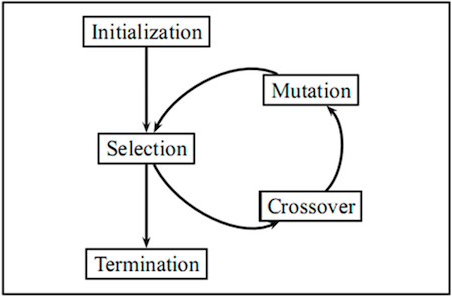
\includegraphics[scale=0.6]{Media/Thing.png}
    \caption{Figure showing the cycle of a genetic algorithm.}
    \label{fig:thing}
\end{figure}
%---------------------------------------------------------------------------
\section{Evolutionary Algorithms in Bioinformatics}
\label{Evolutionary Algorithms in Bioinformatics Section}

This essay explores the applications of evolutionary algorithms in Bioinformatics in RNA structure discovery, motif discovery \cite{Piserchia} and multiple sequence alignment \cite{Radenbaugh}. In the assistance in the discovery of the RNA structure, "an evolutionary algorithm is used to improve each structure based on both free and pseudo-free energies. Finally, a structure with minimum summation of free and pseudo-free energies is considered as the predicted RNA secondary structure." \cite{RNA}. Through combining an evolutionary genetic algorithm and a random projection strategy to identify the (l-d)-Motifs through deduction of potential candidate Motifs to which can be applied to a fitness function \cite{Motif}, also "helps us distinguish real signal sub sequence patterns from background sequences"\cite{Wong}. In the area of multiple sequence alignment, where the similarities between multiple sequences are analyzed \cite{Wong}, genetic algorithms are used to provide the accuracy of the protein alignment for the individual methods used \cite{Multiple1}, further accuracy is theoretically possible using a combination of Markov models and the partition function (particle swarm optimization) \cite{Multiple2}.

\section{Candidate Solution \& the Fitness Function}
\label{Candidate Solution & the Fitness Function Section}

Exploring the assistance in Motif discovery, a candidate solution is derived to the initial population of the genetic algorithm so to improve the range of "candidate motifs" \cite{Motif}. However in the experiment in \cite{Motif}, "Since the search space is large, randomly generated population will rarely come close to an optimal solution and there is little chance that a random population will converge to the optimal solution."\cite{Motif}.

Further exploration into the use of the candidate solution and fitness function in bioinformatics, in multiple sequence alignment, the population ("characterized by four parameters namely, population size, crossover rate, mutation rate, and elitist selection."\cite{Multiple1}) is given a fitness function to produce a population that is based off its individual fitness. Processes such as selection, crossover (random exchange of genetic material between chromosomes) and mutation (random change of a certain bit in a chromosome) are used on the fittest populace, which births form parent to offspring the next generation of the process, which begins again until the termination condition is satisfied. Deeper analysis shows that multiple researchers have applied genetic algorithms, in the software 'SAGA' made by Notredame and Higgins \cite{Multiple3}, "SAGA uses two types of crossover: one-point (shown in \cref{fig:single}) and uniform (shown in \cref{fig:uniform}). It uses 20 different types of complex mutation operators other than two crossover operations to obtain optimum alignment."\cite{Multiple1}. 

\begin{figure}[H]
    \centering
    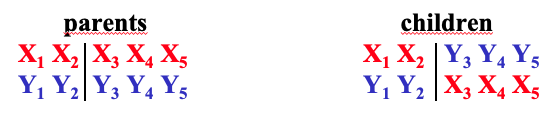
\includegraphics[scale=0.65]{Media/Single.png}
    \caption{Figure showing the parent and children of single-point crossover (crossover point is randomly chosen)}
    \label{fig:single}
\end{figure}

\begin{figure}[H]
    \centering
    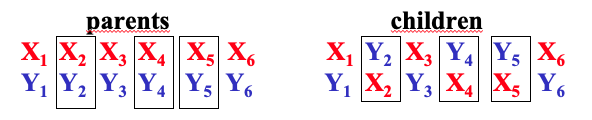
\includegraphics[scale=0.6]{Media/Uniform.png}
    \caption{Figure showing the parent and children of uniform crossover (each gene value is crossed-over with probability $p_c$)}
    \label{fig:uniform}
\end{figure}
%---------------------------------------------------------------------------
\section{Advantages of EA's in Bioinformatics}
\label{Advantages of EA in Bioinformatics Section}

Generic advantages of using the genetic algorithm are improved analysis of a variety of data where the fitness function defines only certain data succeeds into the next repetition in the form of a new data population. The algorithm not only can analyse data regardless of size but also analyse each individual in the total population in terms of a variety of variables. More specific to Bioinformatics, this is important as the size of the data to too vast to analyse conventionally, by applying the algorithm and selecting the variables, the system will analyse the data and output the fittest population based off the variables and terminate accordingly.
%---------------------------------------------------------------------------
\section{Disadvantages of EA's in Bioinformatics}
\label{Disadvantages of EA in Bioinformatics Section}

In Bioinformatics, there appears to be some controversy surrounding the use of evolutionary algorithms as implementing the algorithm, designing a fitness function that is specifically related to the data population and choosing select variables can be difficult, the rates of the crossover and mutation operators can also swing the result to favour a more bias output, more so as this method requires expensive computation compared to conventional methods. The fitness function can only guide the algorithm to achieve a result, a failure in the design would alter a bias result and could be theoretically why evolutionary algorithms are fully trusted yet. Generic disadvantages of using the genetic algorithm is that one must choose a fixed number of iterations by generations or choose a stopping criterion (which can be unknown), more so the choice of operation is in question with crossover wielding a high probability and mutation wielding low probability.
%---------------------------------------------------------------------------
\section{Conclusion}
\label{Conclusion Section}
In conclusion, this essay highlights the structure and the use of the application of evolutionary algorithms (specifically the genetic algorithm) in Bioinformatics, while still controversially used proves to be highly useful in examining large amounts of data which is vastly apparent in Bioinformatics and analyzing the data via a variety of pre-chosen variables. Only used in a few areas within bioinformatics and biology, there is still more uses for these evolutionary algorithms as they have proven to provide solutions based off the strength of its own data that fit the chosen variables, it can be said that these algorithms have a very broad reach in every area of research and experimental testing. It could be said that with an expanse of computational bioinformatics, the use of evolutionary algorithms may rise as the disadvantages outlined in \cref{Disadvantages of EA in Bioinformatics Section} lack trepidation.
%---------------------------------------------------------------------------
\newpage
\bibliographystyle{plain}
\bibliography{mybib.bib}
\end{document}